\documentclass{article}

\usepackage{arxiv}
\usepackage[utf8]{inputenc}
\usepackage[T1]{fontenc}
\usepackage{url}
\usepackage{booktabs}
\usepackage{amsfonts}
\usepackage{nicefrac}
\usepackage{microtype}
\usepackage{graphicx}
\usepackage[font=small,labelfont=bf]{caption}
\usepackage{cite}
\usepackage{pdflscape}
\usepackage{listings}
\usepackage{outlines}
\usepackage{tikz}
\usepackage{epigraph}
\usepackage{natbib} 
\usepackage{url}
\usepackage{algorithm,algpseudocode}

\newcommand*\circled[1]{\tikz[baseline=(char.base)]{
		\node[shape=circle,draw,inner sep=1pt] (char) {#1};}}

\title{Lineage of tiered data in Apache Kafka}

\begin{document}
\maketitle \thispagestyle{fancy2}
\begin{abstract}
	The objective of this document is to elaborate on the design of "tiered storage" to ensure the lineage of logs in Apache Kafka is preserved  when segments are moved to and accessed from external storage tiers.
\end{abstract}

\tableofcontents

\section{Motivation}
\epigraph{\textit{"At its heart a Kafka partition is a replicated log"}}{Apache Kafka online documentation \cite{RD1}}

As stated in the reference documentation and echoed in \cite{KDG}, replication in Apache Kafka is one of its most fundamental characteristic. The replication protocol which Kafka implements and the guarantees it provides are well documented \cite{KIP101} \cite{KIP279}, and explains how and why a consistent lineage for a topic-partition is preserved across its replicas irrespective of the nature and frequency of fail-overs this topic-partition experiences. 

Introducing a feature which would weaken the replication guarantees offered by Kafka is a red herring. Over time, Kafka gracefully evolved and built on top of existing replication protocol to strengthen replication semantic  One of the premise of the integration of data tiering in Apache Kafka is to provide users with a uniform experience of access to data irrespective of its provenance (the storage tier where it comes from). This especially means data lineage is kept consistent when tiered segments are the source of data and the specifications which apply to local replicas are still honored when tiered segments contribute to a replica's lineage.

This document assumes some level of familiarity with the replication protocol implemented in Kafka and how replica lineage is maintained across replicas. At a very high level, this protocol is based on \textit{log truncation}, which relies on replica history, materialized by a list of generation to start offset vectors, which evolves with cluster events and leadership migration. At a given point in time, the lineage of the log of a topic-partition is that of the leader replica of that topic-partition. It is possible for the end offset of the log to decrease when leadership of a topic-partition is migrated.

\section{Introducing example}

The following discussion is based on an example which consists in a topic-partition with three replicas and which experiences leadership migrations. The lineage tree of the topic-partition is provided in diagrams along with the leadership assignments throughout the sequence of generations for this topic-partition.

\subsection{Notations and simplifications}

\textbf{Serialized offsets}

We will informally select offsets from the available replicas at points of interest. An offset is written "$\theta$" and informally indexed such that $\theta_{i+1}$ is written on a replica "after" $\theta_i$ for any given index $i$. The use of leader epochs makes this serialization possible and ensure the word \textit{after} is meaningful in this context. Note that $(\theta_i)_{i \in \mathbb{N}}$ is not necessarily monotonic. 

\textbf{Generations}

A leader epoch is written $g$ and is indexed such that $g_{i+1}$ is "younger" than $g_i$. Note that, for simplicity, the exact sequence of incremental leader epochs is not reproduced. For instance, when replica 2 and 3 go offline in figure \ref{fig:lineage-tree-1}, the leader epoch of the topic-partition is expected to be incremented at least twice, but we will simply refer to the new leader epoch as $g_2$ even if it differs from $g_1$ by more than one logical increment.

\subsection{Lineage tree}

\label{lineage_tree}
\textbf{Figure \ref{fig:lineage-tree-1}} provides the lineage tree of the log, where each replica exhibits a specific history.
The timeline of events which led to this tree are as follows:

\begin{outline}[enumerate]
\1 The root of the tree corresponds to the subsegment in the range $[\theta_1, \theta_2]$, which is assumed to be common to all three replicas.
\1 At generation $g_2$, replicas 2 and 3 become offline and replica 1 ingest records from $\theta_{2} + 1$ to beyond $\theta_3$. The segment with base offset $\theta_1$ and end offset $\theta_3$ is offloaded by replica 1\footnote{Here, the word \textit{replica} informally refers to the hosting \textit{broker}.}. The information required to know how that segment participated to the lineage of the replica needs to be preserved and leader epochs $g_1$ and $g_2$ along with start and end offsets are kept as part of the tiered segment metadata.
\1 Replica 1 becomes offline and replica 2 and 3 now contribute to the ISR set. Replica 3 is the leader. The segment with the offset range $[\theta_1, \theta_4]$ is offloaded and its generational metadata is recorded.
\1 Replica 2 falls behind and is moved out of ISR. Replica 3 continues to ingest and offload the segment ranging from offsets $[\theta_4 + 1, \theta_5]$ at generation $g_4$. This is possible because the ISR is reduced to its leader and the leader high watermark can freely moves forward.
\1 Leadership is transferred to replica 2 and replica 3 is put offline. The ISR set is now $\{2\}$. Data continues to be ingested.
\1 Replica 3 is back online. Generation is incremented to $g_6$ when it joins the cluster. Truncation is performed on the replica, which physically deletes the segment $[\theta_{5}+1, \theta_{5}+2]$. The segment the replica offloaded at generation $g_4$ is only in the external storage at truncation time. This segment is now "\textit{orphan}", because no matter the following life events affecting the cluster, there is no going back and that part of the lineage is forever discarded. Another way to see it is that the edge from the prefix $[\theta_2+1,\theta_4]$ to $[\theta_4+1,\theta_6]$ in the lineage tree can be removed.
\1 The segment $[\theta_2+1,\theta_6]$ is rolled over and eventually become eligible for tiering. It is offloaded by replica 2 and its generational metadata is recorded.
\end{outline}

The content of the tiered storage after these events is represented in \textbf{figure \ref{fig:tiered-storage}}, with the representation of the generational metadata associated to the tiered segments as a graph $\mathcal{G}=(\theta,g)$ which provides the ranges of offsets of the tiered segments along with the leader epochs at ingestion time.

\begin{figure}[H]
	\centering
	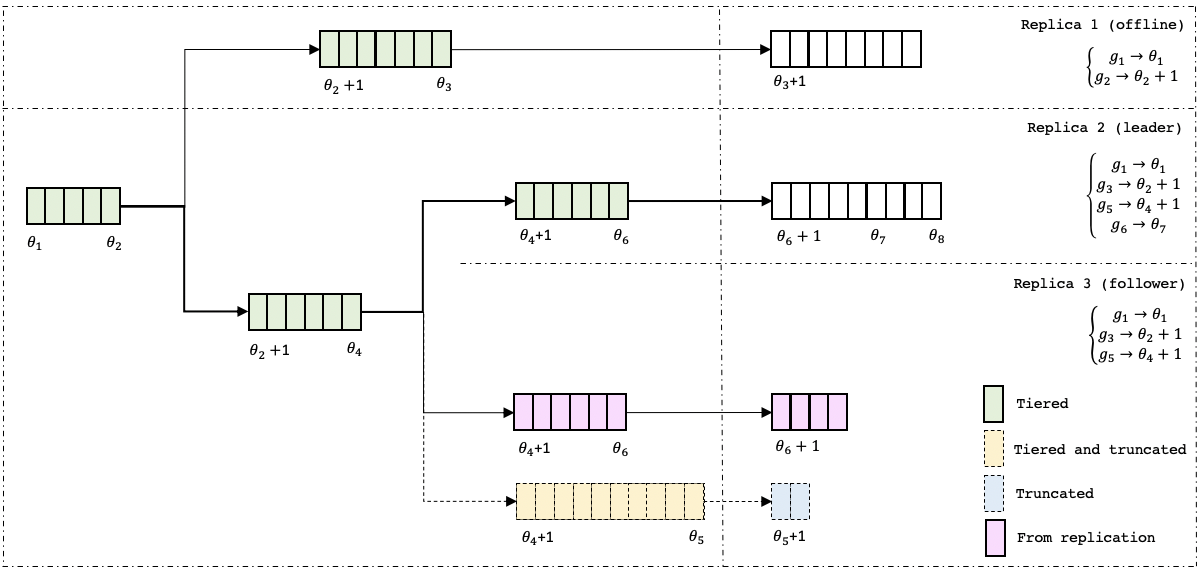
\includegraphics[scale=0.45]{lineage-tree-1.png}
	\captionof{figure}{Lineage tree of the topic-partition while replica 1 is offline. The generation-to-start-offset vectors, which build the leader epoch cache, are represented on the right.}
	\label{fig:lineage-tree-1}
\end{figure}

\begin{figure}[H]
	\centering
	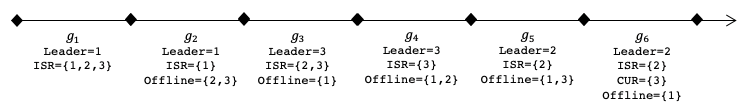
\includegraphics[scale=0.6]{seq-generations.png}
	\captionof{figure}{Lineage tree of the topic-partition while replica 1 is offline.}
	\label{fig:seq-generations}
\end{figure}

\begin{figure}[H]
	\centering
	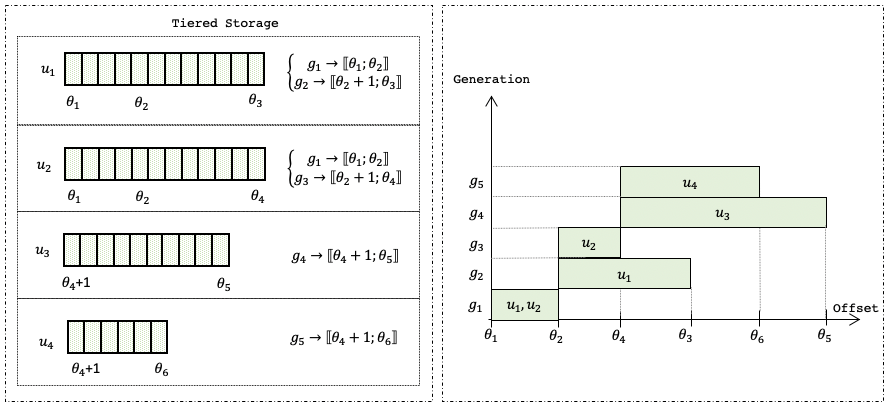
\includegraphics[scale=0.54]{tiered-storage.png}
	\captionof{figure}{On the left: tiered segments. On the right: a representation of lineage information associated to these segments.}
	\label{fig:tiered-storage}
\end{figure}

\newpage
\section{Analysis of lineage reconcilation with tiered segments}

\subsection{Reconcilation between local and tiered segments on \texttt{become-leader}}

\subsubsection{Remote End Offset}

A replica which becomes the leader of a topic-partition, and detects tiered segments for that topic-partition, tries to identify which parts of its lineage are present in the tiered storage. 

A proposed approach is as follows: the replica which becomes a leader will try to find a leader epoch which is common to tiered segments and the local epoch cache, following an approach similar to the resolution of the truncation offset \cite{KIP279}. It then chooses an offset depending on the relative position of the latest offset of the tiered segments and the local end offset.

Multiple outcomes can result. In figure \ref{fig:become-leader}, the following notations are used:

\begin{itemize}
	\item $\theta_R(g)$ is the last offset of all segments, or part of segments, which contain records ingested at generation $g$.
	\item $\theta_S(g)$ is the local start offset for the leader epoch $g$ (inclusive).
	\item $\theta_E(g)$ is the local end offset for the leader epoch $g$ (inclusive).
\end{itemize} 

\begin{figure}[h!]
	\centering
	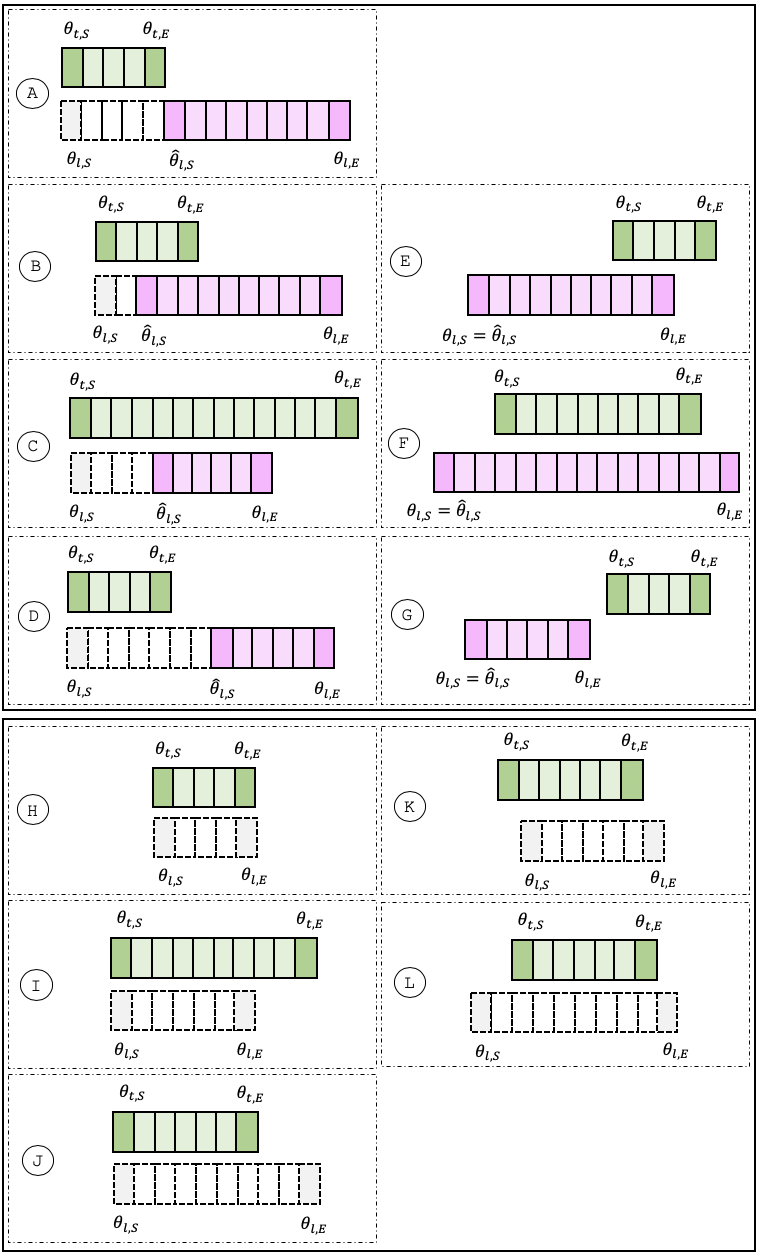
\includegraphics[scale=0.65]{become-leader.png}
	\captionof{figure}{.}
	\label{fig:become-leader}
\end{figure}

\begin{outline}[enumerate]
	\1 \textbf{Case \circled{A}}: A common epoch $g$ exists and $\theta_R(g) = \theta_S(g) - 1$.
	\1 \textbf{Case \circled{B}}:  A common epoch $g$ exists and $\theta_E(g) \geq \theta_R(g) \geq \theta_S(g)$. This can happen for instance if a tiered segment was not deleted on the local replica, and/or the base offsets of the segments of the replica were not perfectly aligned with those of the previous leader, resulting in shifted roll-overs and local segment deletion.
	\1 \textbf{Case \circled{C}}:  A common epoch $g$ exists and $\theta_R(g) > \theta_E(g) \geq \theta_S(g)$. This can happen if the replica was previously out of the ISR set, and uncleanly elected as a leader.
	\1 \textbf{Case \circled{D}}:  A common epoch $g$ exists and $\theta_R(g) < \theta_S(g) - 1$. This could happen in pathological cases, for instance if log retention periods diverge between brokers.
	\1 \textbf{Case \circled{E}}:  No common epoch can be found between tiered segments and the local epochs, no part of the local log is present in the tiered storage. That could be the case that historically, no part of the replica has ever been offloaded \circled{E.1}. However, there could be tiered segments which lineage was removed from the local epoch cache (log prefix truncation via \texttt{LeaderEpochFileCache\#truncateFromStart}) \circled{E.2}.
\end{outline}

In order to handle case \circled{E.2}, the epoch to start offset vectors for the epochs which are fully "tiered" (i.e. for which all segments are in the external storage and do not have remaining local copy) will be preserved. This will be in a file different from the local epoch cache to ensure no conflict can be introduced with existing functionalities.

The new leader will then derive the \textit{remote end offset} (\textbf{REO}), which is relative to a given leader epoch.

\begin{outline}[enumerate]
	\1 \textbf{Case \circled{A}}: The REO can be set to $\theta_R$ (by convention, the REO will be inclusive, if not, $\theta_R = \theta_S +1$ can be adopted).
	\1 \textbf{Case \circled{B}}: The records present simultaneously in the external and local storage are guaranteed to match. The remote end offset will be set to $\theta_R$. Any segment with base offset and end offset within the range $[\theta_S; \theta_R]$ will not be offloaded.
	\1 \textbf{Case \circled{C}}: In this case, we will want to consider the lineage of the new leader to be consistent with the existing behaviour with local segments. The REO will be set to $\theta_E$, and the portion of the log in the range $[\theta_E + 1, \theta_R]$ will not be part of the current lineage (but is not deleted, because it can be reinstated as a part of the log by another leader in the future).
	\1 \textbf{Case \circled{D}}: The REO will be set to $\theta_R$. No assumption should be made in other part of the system that the log concatenated from tiered and local segments is contiguous.
	\1 \textbf{Case \circled{E}}: The REO will be set to $-1$.
\end{outline}

\subsubsection{REO resolution algorithm}

An algorithm to resolve the REO (algorithm \ref{alg:reo}) which derived from the previous discussion is provided here. The following conventions are used:

\begin{itemize}
	\item $\phi$ is a map such that $\phi(g)$ represents the start offset of generation $g$ in the leader epoch cache.
	\item $\psi$ is a map such that $\psi(g)$ represents the end offset of all segments tiered for the generation $g$.
	\item The input of the algorithm are the list of generation to end offset $(g_k, \psi(g_k))_{k \in \{1,...,n\}}$, and the leader epoch cache $(h_l, \phi(h_l))_{l \in \{1,...,m\}}$.
	\item The function \textsc{EpochEndOffset} corresponds to \texttt{LeaderEpochFileCache\#endOffsetFor} and implicitly has access to the map $\phi$.
\end{itemize} 

\begin{algorithm}[h!]
	\caption{Resolution of the replica's REO on \texttt{LeaderAndIsr\#become-leader}}
	\label{alg:reo}
	
	\begin{algorithmic}[1]
		\Function{FindRemoteEndOffset}{$(g_k)_{k \in \{1,..,n\}}$, $\psi$, $(h_h)_{h \in \{1,..,m\}}$, $\phi$}
			\State	$(i,j) \leftarrow (n-1,m-1)$
			\State	$(g_{-1}, h_{-1}) \leftarrow (-1,-1)$
			\\
			\While{$g_i \neq h_j$}
				\While{$g_i > h_j$}
					\State $i \leftarrow i - 1$
				\EndWhile
				\While{$h_j > g_i$}
					\State $j \leftarrow j - 1$
				\EndWhile
			\EndWhile
			\\
			\State // If there is no common lineage, return -1. Note that -1 is already used for sentinel leader epoch in multiple places.
			\State // Need to check conflicting semantic is avoided.
			\If{$i = -1$}
				\State \Return $-1$
			\EndIf
			\\
			\State // Get the latest offset of tiered segments and the local start offset, for the generation $g_i = h_j$.
			\State $\theta_R \leftarrow \psi(g_i)$
			\State $\theta_E \leftarrow  \textsc{EpochEndOffset}(h_j)$
			\\
			\If{$\theta_R > \theta_E$}
			\State \Return $\theta_E - 1$ // Case \circled{C}
			\Else
			\State \Return $\theta_R$ // Case \circled{A}, \circled{B}, \circled{D}
			\EndIf
			\\
		\EndFunction
	\end{algorithmic}	
\end{algorithm}


\subsection{Reconciliation between local and tiered segments on \texttt{become-follower}}

When a replica initiates replication from a leader, it needs to know which part of its lineage is tiered, to avoid replicating it from the leader, or expecting the tiered segments not be found locally. This requires two things:

\begin{outline}[enumerate]
\1 Reconciliate its local segments with the lineage $\mathcal{L}$ of the leader it replicates from. This is implemented with the truncation protocol.
\1 Reconciliate 
\end{outline}


All the follower need to know is the last offset of the latest tiered segment according to the current replica lineage. In the case of the lineage tree in figure \ref{fig:lineage-tree-1}, that would be $\theta_6$. Note that this is not necessarily the \textit{latest} segment offloaded, nor the largest offset of all the segments offloaded for that topic-partition ($\theta_6 < \theta_5$).

Consider the example described in section \ref{lineage_tree}. 

\newpage
\section{Garbage collection of orphan segments}

\newpage
\bibliographystyle{plain}
\bibliography{tiered-storage-replication}{}
\end{document}
